\documentclass{standalone}
\usepackage{tikz}
\usetikzlibrary{patterns, positioning}
\usepackage[sfdefault]{ClearSans} %% option 'sfdefault' activates Clear Sans as the default text font
\usepackage[T1]{fontenc}

\begin{document}
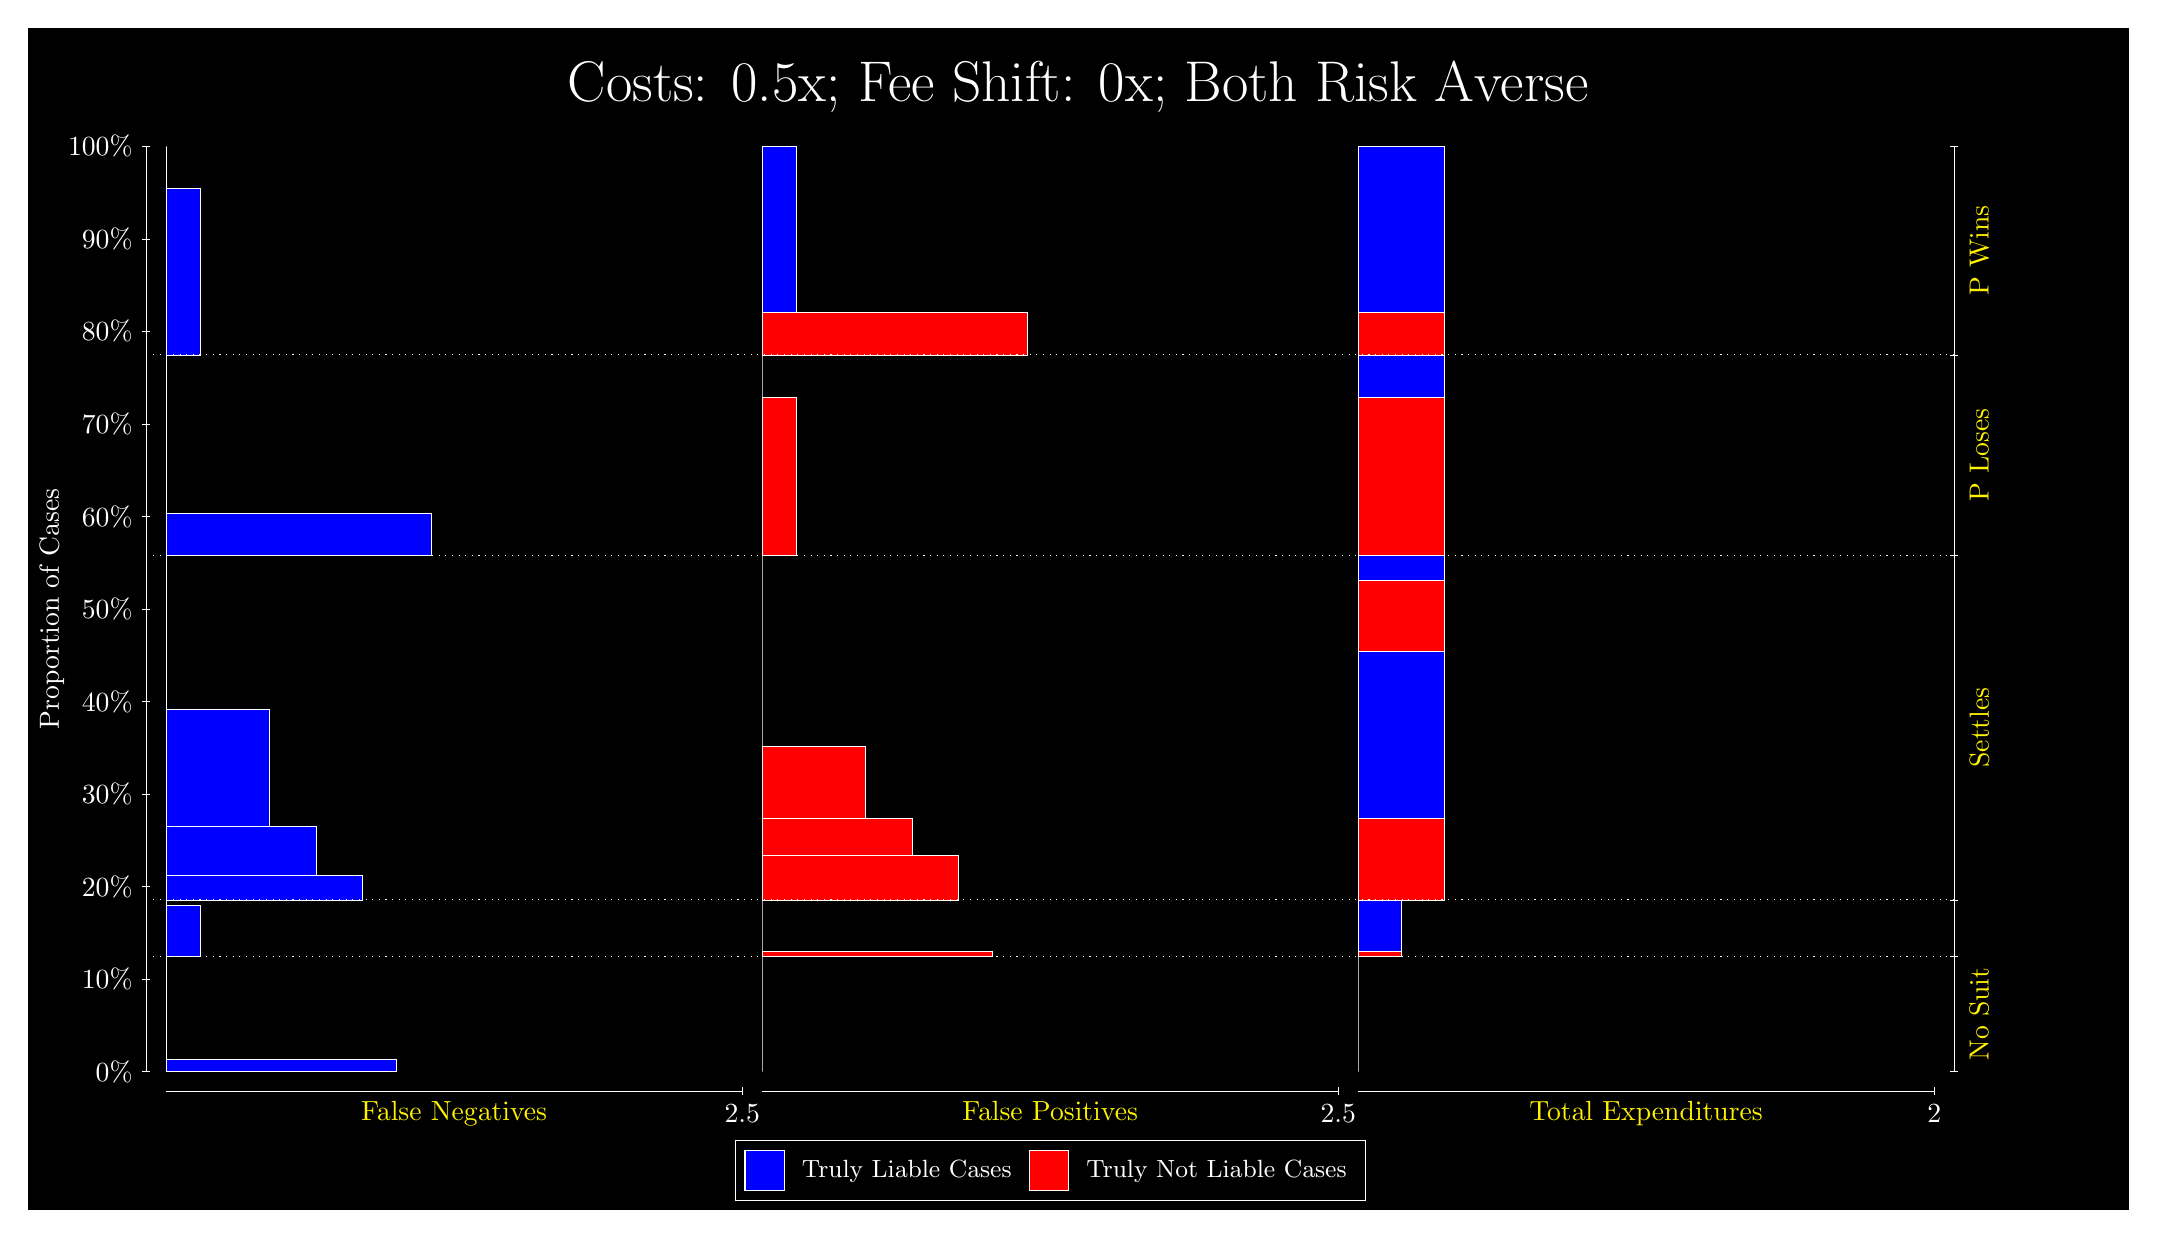
\begin{tikzpicture}
\draw[fill=black] (0,0) rectangle (26.667,15);
\draw[text=white] (0,13.5) rectangle (26.667,15) node[midway] {\huge Costs: 0.5x; Fee Shift: 0x; Both Risk Averse};
\draw[white, very thin] (1.5,1.75) -- (1.5,13.5);
\node[rotate=90, text=white, anchor=center] at (0.3, 7.625) {Proportion of Cases};
\draw[white, very thin] (1.45,1.75) -- (1.55,1.75);
\node[text=white, anchor=east] at (1.45, 1.75) {0\%};
\draw[white, very thin] (1.45,2.925) -- (1.55,2.925);
\node[text=white, anchor=east] at (1.45, 2.925) {10\%};
\draw[white, very thin] (1.45,4.1) -- (1.55,4.1);
\node[text=white, anchor=east] at (1.45, 4.1) {20\%};
\draw[white, very thin] (1.45,5.275) -- (1.55,5.275);
\node[text=white, anchor=east] at (1.45, 5.275) {30\%};
\draw[white, very thin] (1.45,6.45) -- (1.55,6.45);
\node[text=white, anchor=east] at (1.45, 6.45) {40\%};
\draw[white, very thin] (1.45,7.625) -- (1.55,7.625);
\node[text=white, anchor=east] at (1.45, 7.625) {50\%};
\draw[white, very thin] (1.45,8.8) -- (1.55,8.8);
\node[text=white, anchor=east] at (1.45, 8.8) {60\%};
\draw[white, very thin] (1.45,9.975) -- (1.55,9.975);
\node[text=white, anchor=east] at (1.45, 9.975) {70\%};
\draw[white, very thin] (1.45,11.15) -- (1.55,11.15);
\node[text=white, anchor=east] at (1.45, 11.15) {80\%};
\draw[white, very thin] (1.45,12.325) -- (1.55,12.325);
\node[text=white, anchor=east] at (1.45, 12.325) {90\%};
\draw[white, very thin] (1.45,13.5) -- (1.55,13.5);
\node[text=white, anchor=east] at (1.45, 13.5) {100\%};

\draw[white, very thin] (24.457,1.75) -- (24.457,13.5);
\draw[white, very thin] (24.407,1.75) -- (24.507,1.75);
\node[anchor=west] at (24.407, 1.75) {};
\draw[white, very thin] (24.407,3.2075) -- (24.507,3.2075);
\node[anchor=west] at (24.407, 3.2075) {};
\draw[white, very thin] (24.407,3.931) -- (24.507,3.931);
\node[anchor=west] at (24.407, 3.931) {};
\draw[white, very thin] (24.407,8.3068) -- (24.507,8.3068);
\node[anchor=west] at (24.407, 8.3068) {};
\draw[white, very thin] (24.407,10.851) -- (24.507,10.851);
\node[anchor=west] at (24.407, 10.851) {};
\draw[white, very thin] (24.407,13.5) -- (24.507,13.5);
\node[anchor=west] at (24.407, 13.5) {};

\draw[white, very thin, fill=blue] (1.75,1.75) rectangle (4.6775,1.9033);
\draw[white, very thin, fill=red] (1.75,1.9033) rectangle (1.75,3.2075);
\draw[white, very thin, fill=blue] (1.75,3.2075) rectangle (2.1891,3.857);
\draw[white, very thin, fill=red] (1.75,3.857) rectangle (1.75,3.931);
\draw[white, very thin, fill=blue] (1.75,3.931) rectangle (4.2384,4.2429);
\draw[white, very thin, fill=blue] (1.75,4.2429) rectangle (3.6529,4.8623);
\draw[white, very thin, fill=blue] (1.75,4.8623) rectangle (3.0674,6.3554);
\draw[white, very thin, fill=red] (1.75,6.3554) rectangle (1.75,8.3068);
\draw[white, very thin, fill=blue] (1.75,8.3068) rectangle (5.1167,8.8425);
\draw[white, very thin, fill=red] (1.75,8.8425) rectangle (1.75,10.851);
\draw[white, very thin, fill=blue] (1.75,10.851) rectangle (2.1891,12.963);
\draw[white, very thin, fill=red] (1.75,12.963) rectangle (1.75,13.5);
\draw[white, very thin, fill=red] (9.3189,1.75) rectangle (9.3189,3.0542);
\draw[white, very thin, fill=blue] (9.3189,3.0542) rectangle (9.3189,3.2075);
\draw[white, very thin, fill=red] (9.3189,3.2075) rectangle (12.246,3.2816);
\draw[white, very thin, fill=blue] (9.3189,3.2816) rectangle (9.3189,3.931);
\draw[white, very thin, fill=red] (9.3189,3.931) rectangle (11.807,4.4924);
\draw[white, very thin, fill=red] (9.3189,4.4924) rectangle (11.222,4.9717);
\draw[white, very thin, fill=red] (9.3189,4.9717) rectangle (10.636,5.8825);
\draw[white, very thin, fill=blue] (9.3189,5.8825) rectangle (9.3189,8.3068);
\draw[white, very thin, fill=red] (9.3189,8.3068) rectangle (9.758,10.315);
\draw[white, very thin, fill=blue] (9.3189,10.315) rectangle (9.3189,10.851);
\draw[white, very thin, fill=red] (9.3189,10.851) rectangle (12.686,11.388);
\draw[white, very thin, fill=blue] (9.3189,11.388) rectangle (9.758,13.5);
\draw[white, very thin, fill=red] (16.888,1.75) rectangle (16.888,3.0542);
\draw[white, very thin, fill=blue] (16.888,3.0542) rectangle (16.888,3.2075);
\draw[white, very thin, fill=red] (16.888,3.2075) rectangle (17.437,3.2816);
\draw[white, very thin, fill=blue] (16.888,3.2816) rectangle (17.437,3.931);
\draw[white, very thin, fill=red] (16.888,3.931) rectangle (17.986,4.9717);
\draw[white, very thin, fill=blue] (16.888,4.9717) rectangle (17.986,7.0842);
\draw[white, very thin, fill=red] (16.888,7.0842) rectangle (17.986,7.995);
\draw[white, very thin, fill=blue] (16.888,7.995) rectangle (17.986,8.3068);
\draw[white, very thin, fill=red] (16.888,8.3068) rectangle (17.986,10.315);
\draw[white, very thin, fill=blue] (16.888,10.315) rectangle (17.986,10.851);
\draw[white, very thin, fill=red] (16.888,10.851) rectangle (17.986,11.388);
\draw[white, very thin, fill=blue] (16.888,11.388) rectangle (17.986,13.5);
\draw[white, dotted] (1.5,3.2075) -- (24.457,3.2075);
\draw[white, dotted] (1.5,3.931) -- (24.457,3.931);
\draw[white, dotted] (1.5,8.3068) -- (24.457,8.3068);
\draw[white, dotted] (1.5,10.851) -- (24.457,10.851);
\draw[white, very thin] (1.75,1.5) -- (9.0689,1.5);
\node[text=yellow, anchor=north] at (5.4094, 1.5) {False Negatives};
\draw[white, very thin] (9.0689,1.45) -- (9.0689,1.55);
\node[text=white, anchor=north] at (9.0689, 1.45) {2.5};

\draw[white, very thin] (9.3189,1.5) -- (16.638,1.5);
\node[text=yellow, anchor=north] at (12.978, 1.5) {False Positives};
\draw[white, very thin] (16.638,1.45) -- (16.638,1.55);
\node[text=white, anchor=north] at (16.638, 1.45) {2.5};

\draw[white, very thin] (16.888,1.5) -- (24.207,1.5);
\node[text=yellow, anchor=north] at (20.547, 1.5) {Total Expenditures};
\draw[white, very thin] (24.207,1.45) -- (24.207,1.55);
\node[text=white, anchor=north] at (24.207, 1.45) {2};

\node[text=yellow, centered, rotate=90] at (24.777, 2.4788) {No Suit};

\node[text=yellow, centered, rotate=90] at (24.777, 6.1189) {Settles};
\node[text=yellow, centered, rotate=90] at (24.777, 9.5789) {P Loses};
\node[text=yellow, centered, rotate=90] at (24.777, 12.176) {P Wins};

\draw (12.978300999999998,1.5) node[draw=none] (baseCoordinate) {};
\begin{scope}[align=center]
        \matrix[scale=0.5, draw=white, below=0.5cm of baseCoordinate, nodes={draw}, column sep=0.1cm]{
            \node[rectangle, draw, minimum width=0.5cm, minimum height=0.5cm, fill=blue] {}; &
            \node[draw=none, font=\small, text=white] (B) {Truly Liable Cases}; &
            \node[rectangle, draw, minimum width=0.5cm, minimum height=0.5cm, fill=red] {}; &
            \node[draw=none, font=\small, text=white] (B) {Truly Not Liable Cases}; \\
            };
\end{scope}

\end{tikzpicture}
\end{document}